\section{Policy Gradient Theorem}\label{PGTsection}

\subsection{Вывод первым способом}

Часто говорят, что функционал в задаче обучения с подкреплением не дифференцируем. Имеется в виду, что функция награды $r(s, a)$ не дифференцируема по действиям $a$; например, просто потому что пространство действий дискретно, например, в состоянии $s$ агент выбрал действие $a \HM = 0$ и значение полученной награды можно лишь сравнивать со значениями для других действий. Однако, мы уже видели в примере \ref{ex:score}, что это не мешает дифференцируемости по параметрам стратегии в ситуации, когда стратегия ищется в семейсте стохастичных стратегий. Фактически, оптимизация в пространстве стохастичных стратегий является этакой <<релаксацией>> нашей задачи.

Пусть политика $\pi_{\theta}(a \mid s)$ параметризована $\theta$ и дифференцируема по параметрам. Тогда наш оптимизируемый функционал $J(\pi) \HM= V^\pi(s_0)$ тоже дифференцируем по $\theta$, и далее мы будем выводить формулу этого градиента. Для этого нам понадобится стандартная техника вычисления градиента мат.ожидания по распределению, зависящего от параметров; мы уже встречались с ней при обсуждении эволюционных стратегий в главе \ref{subsec:nes}. Сейчас в оптимизируемом функционале у нас стоит целая цепочка вложенных мат.ожиданий, и наш вывод будет заключаться просто в последовательном применении той же техники к каждому стоящему там мат.ожиданию $\E_{a \sim \pi(a \mid s)} ( \cdot )$.

Заранее оговоримся, что при минимальных технических условиях регулярности\footnote{это следует из наших условий регулярности на MDP и предположения интегрируемости всех функций; тогда все оценочные функции и награды ограничены, следовательно, все интегралы и ряды в рассуждении сходятся абсолютно и равномерно по параметрам $\theta$; мы просто не <<связываемся>> в контексте нашей задачи с бесконечностью, на которой в теории математического анализа и возникают ситуации, когда так делать нельзя.} мы имеем право менять местами знаки градиента, мат.ожиданий, сумм и интегралов.

\begin{theorem}
\begin{equation}\label{Vgrad}
\nabla_{\theta} V^{\pi}(s) = \E_{a} \left[ \nabla_{\theta} \log \pi_\theta (a \mid s) Q^{\pi}(s, a) + \nabla_{\theta} Q^{\pi}(s, a) \right]
\end{equation}
\beginproof
\begin{align*}
\nabla_{\theta} V^{\pi}(s) &= \{ \text{\eqref{VQ}} \} = \nabla_{\theta} \E_{a} Q^{\pi}(s, a) = \\
&= \{ \text{мат.ожидание --- это интеграл} \} = \\
&= \nabla_{\theta} \int\limits_{\A} \pi_\theta(a \mid s) Q^{\pi}(s, a) \diff a = \\
&= \{ \text{проносим градиент внутрь интеграла} \} = \\
&= \int\limits_{\A} \nabla_{\theta} \left[ \pi_\theta(a \mid s) Q^{\pi}(s, a) \right] \diff a = \\
&= \{ \text{правило градиента произведения} \} = \\
&= \int\limits_{\A} \nabla_{\theta} \pi_\theta(a \mid s) Q^{\pi}(s, a) \diff a + \int\limits_{\A} \pi_\theta(a \mid s) \nabla_{\theta} Q^{\pi}(s, a) \diff a = \\
&= \{ \text{второе слагаемое --- это мат.ожидание} \} = \\
&= \int\limits_{\A} \nabla_{\theta} \pi_\theta(a \mid s) Q^{\pi}(s, a) \diff a + \E_{a} \nabla_{\theta} Q^{\pi}(s, a) = \\
&= \{ \text{log-derivative trick \eqref{logderivtrick}} \} = \\
&= \int\limits_{\A} \pi_\theta(a \mid s) \nabla_{\theta} \log \pi_\theta(a \mid s) Q^{\pi}(s, a) \diff a + \E_{a} \nabla_{\theta} Q^{\pi}(s, a) = \\
&= \{ \text{первое слагаемое тоже стало мат.ожиданием} \} = \\
&= \E_{a} \left[ \nabla_{\theta} \log \pi_\theta(a \mid s) Q^{\pi}(s, a) + \nabla_{\theta} Q^{\pi}(s, a) \right] \tagqed
\end{align*}
\end{theorem}

Эта техника вычисления градиента через <<стохастичный узел нашего вычислительного графа>>, когда мы сэмплируем $a \HM \sim \pi(a \HM\mid s)$, носит название REINFORCE. Как видно, эта техника универсальна: применима всегда для любых пространств действий, а также в ситуации, когда функция $Q^{\pi}(s, a)$ не дифференцируема по действиям. Заметим, что в глубоком обучении при некоторых дополнительных условиях в подобных ситуациях бывает также применим другой способ, называемый репараметризационным трюком; его мы обсудим позже в главе \ref{continuouscontrolchapter}, когда пространство действий будет непрерывно, а $Q^{\pi}(s, a)$ --- дифференцируема по действиям, то есть будут выполнены эти самые дополнительные условия. 

Мы смогли выразить градиент V-функции через градиент Q-функции, попробуем сделать наоборот. Для этого нам нужно посчитать градиент от мат.ожидания по функции переходов, не зависящей от параметров нашей стратегии, поэтому здесь всё тривиально. 

\begin{theorem}
\begin{equation}\label{Qgrad}
\nabla_{\theta} Q^{\pi}(s, a) = \gamma \E_{s'} \nabla_{\theta} V^{\pi}(s')
\end{equation}
\beginproof
\begin{align*}
\nabla_{\theta} Q^{\pi}(s, a) &= \{ \text{\eqref{QV}} \} = \nabla_{\theta} \left[ r(s, a) + \gamma \E_{s'} V^{\pi}(s') \right] = \\
&= \{ \text{$r(s, a)$ не зависит от $\theta$, $p(s' \mid s, a)$ тоже} \} = \\
&= \gamma \E_{s'} \nabla_{\theta} V^{\pi}(s')  \tagqed
\end{align*}
\end{theorem}

Подставляя \eqref{Qgrad} в \eqref{Vgrad}, получаем:

\begin{proposition}
\begin{equation}
\nabla_{\theta} V^{\pi}(s) = \E_{a} \E_{s'} \left[ \nabla_{\theta} \log \pi_\theta (a \mid s) Q^{\pi}(s, a) + \gamma \nabla_{\theta} V^{\pi}(s') \right]
\end{equation}
\end{proposition}

Следовательно, мы получили рекурсивное выражение градиента $V^\pi(s)$ через него же само. Очень похоже на уравнение Беллмана, кстати: в правой части стоит мат.ожидание по выбранному в $s$ действию $a$ и следующему состоянию.

Осталось раскрутить эту рекурсивную цепочку, продолжая раскрывать $\nabla_{\theta} V^{\pi}(s')$ в будущее до бесконечности. Аккуратно собирая слагаемые, а также собирая из мат.ожиданий мат.ожидание по траектории, получаем следующее:

\begin{proposition}[Policy Gradient Theorem] Выражение для градиента оптимизируемого функционала можно записать следующим образом:
\begin{equation}\label{pgt_firstproof}
\nabla_{\theta} J(\pi) = \E_{\Traj \sim \pi} \sum_{t \ge 0} \gamma^t \nabla_{\theta} \log \pi_\theta (a_t \mid s_t) Q^{\pi}(s_t, a_t)
\end{equation}
\end{proposition}

\subsection{Вывод вторым способом}

Прежде, чем мы обсудим физический смысл полученной формулы, выведем её альтернативным способом. Применим REINFORCE не к мат.ожиданиям по отдельным действиям, а напрямую к распределению всей траектории следующим образом:

\begin{theorem}
\begin{equation*}
\nabla_{\theta} V^{\pi}(s) = \E_{\Traj \sim \pi} \sum_{t \ge 0} \nabla_{\theta} \log \pi_\theta (a_t \mid s_t) R(\Traj)
\end{equation*}
\begin{proof}
\begin{align*}
\nabla_{\theta} V^{\pi}(s) &= \nabla_{\theta} \E_{\Traj \sim \pi} R(\Traj) = \\
&= \{ \text{рассмотрим мат.ожидание как интеграл по всевозможным траекториям} \} = \\
&= \nabla_{\theta} \iint\limits_{\Traj} p\left( \Traj \mid \pi \right) R(\Traj) \diff \Traj = \\
&= \{ \text{проносим градиент внутрь интеграла} \} = \\
&= \iint\limits_{\Traj} \nabla_{\theta} p\left( \Traj \mid \pi \right) R(\Traj) \diff \Traj = \\
&= \{ \text{log-derivative trick \eqref{logderivtrick}} \} = \\
&= \E_{\Traj \sim \pi} \nabla_{\theta} \log p\left( \Traj \mid \pi \right) R(\Traj) = \\
&= \{ \text{вспоминаем, что вероятность траектории есть произведение вероятностей} \} = \\
&= \E_{\Traj \sim \pi} \sum_{t \ge 0} \nabla_{\theta} \log \pi_\theta (a_t \mid s_t) R(\Traj)
\end{align*}
В последнем переходе логарифмы вероятностей переходов $\sum\limits_{t \ge 0} \nabla_{\theta} \log p(s_{t+1} \mid s_t, a_t)$ сократились как не зависящие от параметров стратегии.
\end{proof}
\end{theorem}

Видим, что мы более простым способом получили очень похожую формулу, но с суммарной наградой за игры вместо Q-функции из первого доказательства \eqref{pgt_firstproof}. В силу корректности всех вычислений, уже можно утверждать равенство между этими формулами, что наводит на мысль, что градиент можно записывать в нескольких математически эквивалентных формах. Математически эти формы будут эквивалентны, то есть равны, как интегралы, но их Монте-Карло оценки могут начать вести себя совершенно по-разному. Может быть, мы можем как-то <<хорошую форму>> выбрать для наших алгоритмов.

Рассмотрим, как можно этим вторым способом рассуждений дойти формально до формы градиента из первого способа. Раскрывая $R(\Traj)$ по определению, мы сейчас имеем произведение двух сумм под интегралом:
$$\nabla_{\theta} V^{\pi}(s) = \E_{\Traj \sim \pi} \left(\sum_{t \ge 0} \nabla_{\theta} \log \pi_\theta (a_t \mid s_t) \right) \left( \sum_{t' \ge 0} \gamma^{t'} r_{t'} \right)$$

Давайте перемножим эти два ряда:
\begin{equation}\label{fulltwosums}
\nabla_{\theta} V^{\pi}(s) = \E_{\Traj \sim \pi} \sum_{t \ge 0} \sum_{t' \ge 0} \nabla_{\theta} \log \pi_\theta (a_t \mid s_t) \gamma^{t'} r_{t'}
\end{equation}

Видим странную вещь: на градиент по параметрам за решение выбрать $a_t$ в момент времени $t$ влияет награда, собранная при $t' \HM< t$, то есть величина, на которую наше решение точно не могло повлиять, поскольку принималось после её получения. Но почему формально это так?

\begin{theorem}
Для произвольного распределения $\pi_{\theta}(a)$ с параметрами $\theta$, верно:
\begin{equation}\label{baseline}
\,
\E_{a \sim \pi_{\theta}(a)} \nabla_\theta \log \pi_{\theta}(a) = 0 
\end{equation}
\beginproof
\begin{align*}
\E_{a \sim \pi_{\theta}(a)} \nabla_\theta \log \pi_{\theta}(a) &= \{ \text{производная логарифма} \} 
= \E_{a \sim \pi_{\theta}(a)} \frac{\nabla_\theta \pi_{\theta}(a)}{\pi_{\theta}(a)} = \\
&= \int\limits_\A \nabla_\theta \pi_{\theta}(a) \diff a = \nabla_\theta \int\limits_\A \pi_{\theta}(a) \diff a
= \nabla_\theta 1 = 0 \tagqed
\end{align*}
\end{theorem}

Следующее утверждение формализует этот тезис о том, что <<будущее не влияет на прошлое>>: выбор действий в некоторый момент времени никак не влияет на те слагаемые из награды, которые были получены в прошлом.

\begin{proposition} 
При $t > t'$:
\begin{equation*}
\E_{\Traj \sim \pi} \nabla_{\theta} \log \pi_\theta (a_t \mid s_t) \gamma^{t'} r_{t'} = 0
\end{equation*}
\beginproof
\begin{align*}
&\E_{\Traj \sim \pi} \nabla_{\theta} \log \pi_\theta (a_t \mid s_t) \gamma^{t'} r_{t'} = \\
&= \{ \text{представляем мат.ожидание по траектории как вложенные мат.ожидания} \} = \\
&= \E_{a_1, s_1 \dots s_{t'}, a_{t'}} \E_{s_{t'+1}, a_{t'+1} \dots s_t, a_t \dots} \nabla_{\theta} \log \pi_\theta (a_t \mid s_t) \gamma^{t'} r_{t'} = \\
&= \{ \text{выносим константу из мат.ожидания} \} = \\
&= \E_{a_1, s_1 \dots s_{t'}, a_{t'}} \gamma^{t'} r_{t'} \E_{s_{t'+1}, a_{t'+1} \dots s_t, a_t \dots} \nabla_{\theta} \log \pi_\theta (a_t \mid s_t) = \\
&= \{ \text{мат.ожидание градиента логарифма вероятности есть ноль \eqref{baseline}} \} = \\
&= \E_{a_1, s_1 \dots s_{t'}, a_{t'}} \gamma^{t'} r_{t'} \cdot 0 = 0   \tagqed
\end{align*}
\end{proposition}

Значит, вместо полной награды за игру можно в весах оставить только reward-to-go \eqref{rewardtogo}, поскольку из всех слагаемых в \eqref{fulltwosums} слагаемые для $t' \HM< t$ занулятся. Понятно, что дисперсия Монте-Карло оценки такого интеграла будет меньше: мы убрали некоторую зашумляющую часть нашей стохастической оценки, которая, как мы теперь поняли, в среднем равна нулю.

При этом дисконтирование в сумме наград шло с самого начала игры, поэтому для того, чтобы записать формулу в терминах reward-to-go, нужно вынести $\gamma^t$:
$$\sum_{t'=t} \gamma^{t'} r_{t'} = \gamma^t \sum_{t'=t} \gamma^{t' - t} r_{t'} = \gamma^t R_t$$

\begin{proposition}
\begin{equation}\label{reinforce_grad}
\nabla_{\theta} V^{\pi}(s) = \E_{\Traj \sim \pi} \sum_{t \ge 0} \gamma^t \nabla_{\theta} \log \pi_\theta (a_t \mid s_t) R_t
\end{equation}
\end{proposition}

Reward-to-go очень похож на Q-функцию, так как является Монте-Карло оценкой Q-функции, а мат.ожидание по распределениям всё равно берётся. Формальное обоснование эквивалентности выглядит так:

\begin{proposition} Формула \eqref{reinforce_grad} эквивалентна
\begin{equation*}
\nabla_{\theta} V^{\pi}(s) = \E_{\Traj \sim \pi} \sum_{t \ge 0} \gamma^t \nabla_{\theta} \log \pi_\theta (a_t \mid s_t) Q^{\pi}(s_t, a_t)
\end{equation*}
\beginproof
\begin{align*}
\nabla_{\theta} V^{\pi}(s) &= \E_{\Traj \sim \pi} \sum_{t \ge 0} \gamma^t \nabla_{\theta} \log \pi_\theta (a_t \mid s_t) R_t = \\
&= \{ \text{меняем местами сумму по $t$ и мат.ожидание по траекториям} \} = \\
&= \sum_{t \ge 0} \E_{\Traj \sim \pi} \gamma^t \nabla_{\theta} \log \pi_\theta (a_t \mid s_t) R_t = \\
&= \{ \text{представляем мат.ожидание по траектории как вложенные мат.ожидания} \} = \\
&= \sum_{t \ge 0} \E_{a_0, s_1 \dots s_t, a_t} \E_{s_{t+1}, a_{t+1} \dots} \gamma^t \nabla_{\theta} \log \pi_\theta (a_t \mid s_t) R_t = \\
&= \{ \text{выносим константу из мат.ожидания} \} = \\
&= \sum_{t \ge 0} \E_{a_0, s_1 \dots s_t, a_t} \gamma^t \nabla_{\theta} \log \pi_\theta (a_t \mid s_t)  \E_{s_{t+1}, a_{t+1} \dots} R_t = \\
&= \{ \text{видим определение Q-функции} \} = \\
&= \sum_{t=0} \E_{a_0, s_1 \dots s_t, a_t} \gamma^t \nabla_{\theta} \log \pi_\theta (a_t \mid s_t) Q^\pi(s_t, a_t) = \\
&= \{ \text{формально, берём фиктивное мат.ожидание} \} = \\
&= \sum_{t=0} \E_{\Traj \sim \pi} \gamma^t \nabla_{\theta} \log \pi_\theta (a_t \mid s_t) Q^\pi(s_t, a_t) = \\
&= \{ \text{снова меняем местами сумму и мат.ожидание} \} = \\
&= \E_{\Traj \sim \pi} \sum_{t=0} \gamma^t \nabla_{\theta} \log \pi_\theta (a_t \mid s_t) Q^\pi(s_t, a_t)  \tagqed
\end{align*}
\end{proposition}

Итак, мы получили формулу \eqref{pgt_firstproof} вторым способом.

\subsection{Физический смысл}

Обсудим, а в каком направлении, собственно, указывает полученная формула градиента \eqref{pgt_firstproof}. Оказывается, градиент нашего функционала имеет вид градиента взвешенных логарифмов правдоподобий. Чтобы ещё лучше увидеть это, рассмотрим \emph{суррогатную функцию} (surrogate objective) --- другой функционал, который будет иметь в точке текущих значений параметров стратегии $\pi$ такой же градиент, как и $J(\theta)$:
\begin{equation}\label{surrogateobj}
\mathcal{L}_{\textcolor{ChadPurple}{\tilde{\pi}}}(\textcolor{ChadBlue}{\theta}) \coloneqq \E_{\Traj \sim \textcolor{ChadPurple}{\tilde{\pi}(s)}} \sum_{t \ge 0} \gamma^t \log \textcolor{ChadBlue}{\pi_{\theta}}(a \mid s) Q^{\textcolor{ChadPurple}{\tilde{\pi}}}(s, a)
\end{equation}

Это суррогатная функция от двух стратегий: стратегии $\textcolor{ChadBlue}{\pi_{\theta}}$, которую мы оптимизируем, и ещё одной стратегии $\textcolor{ChadPurple}{\tilde{\pi}}$. Давайте рассмотрим эту суррогатную функцию в точке $\theta$ такой, что эти две стратегии совпадают: $\textcolor{ChadPurple}{\tilde{\pi}} \HM\equiv \textcolor{ChadBlue}{\pi_{\theta}}$, и посмотрим на градиент при изменении $\theta$, только одной из них. То есть что мы сказали: давайте <<заморозим>> оценочную Q-функцию, и <<заморозим>> распределение, из которого приходят пары $s, a$. Тогда:

\begin{proposition}
$$\left. \textcolor{ChadBlue}{\nabla_{\theta}} \mathcal{L}_{\textcolor{ChadPurple}{\tilde{\pi}}}(\textcolor{ChadBlue}{\theta}) \right|_{\textcolor{ChadPurple}{\tilde{\pi}} = \textcolor{ChadBlue}{\pi_{\theta}}} = \nabla_{\theta} J(\theta)$$
\begin{proof}
Поскольку мат.ожидание по траекториям не зависит в этой суррогатной функции от $\theta$, то градиент просто можно пронести внутрь:
$$\left. \textcolor{ChadBlue}{\nabla_{\theta}} \mathcal{L}_{\textcolor{ChadPurple}{\tilde{\pi}}}(\textcolor{ChadBlue}{\theta}) \right|_{\textcolor{ChadPurple}{\tilde{\pi}} = \textcolor{ChadBlue}{\pi_{\theta}}} = \E_{\Traj \sim \textcolor{ChadPurple}{\tilde{\pi}(s)}} \sum_{t \ge 0} \gamma^t \left. \textcolor{ChadBlue}{\nabla_{\theta}} \log \textcolor{ChadBlue}{\pi_{\theta}}(a \mid s) \right|_{\textcolor{ChadPurple}{\tilde{\pi}} = \textcolor{ChadBlue}{\pi_{\theta}}} Q^{\textcolor{ChadPurple}{\tilde{\pi}}}(s, a)$$

В точке $\theta \colon \textcolor{ChadPurple}{\tilde{\pi}} \HM= \textcolor{ChadBlue}{\pi_{\theta}}$ верно, что $p(\Traj \HM\mid \textcolor{ChadPurple}{\tilde{\pi}}) \HM\equiv p(\Traj \HM\mid \textcolor{ChadBlue}{\pi})$ и $Q^{\textcolor{ChadPurple}{\tilde{\pi}}}(s, a) \HM = Q^{\textcolor{ChadBlue}{\pi}}(s, a)$; следовательно, значение градиента в этой точке совпадает со значением формулы \eqref{pgt_firstproof}.
\end{proof}
\end{proposition}

Значит, направление максимизации $J(\theta)$ в текущей точке $\theta$ просто совпадает с направлением максимизации этой суррогатной функции! Это принципиально единственное свойство введённой суррогатной функции. Таким образом, можно считать, что в текущей точке мы на самом деле <<как бы>> максимизируем \eqref{surrogateobj}, а это уже в чистом виде логарифм правдоподобия каких-то пар $(s, a)$, для каждой из которых дополнительно выдан <<вес>> в виде значения $Q^{\pi}(s, a)$.

\begin{remark}
Эта суррогатная функция очень удобна для подсчёта градиента $\nabla_\theta J(\pi)$, поскольку она представляет его <<в терминах лосса>>:
$$\nabla_\theta J(\pi) = \nabla_\theta \Loss^{\actor}(\theta)$$
Это полезно в средствах автоматического дифференцирования, где нужно задать некоторый вычислительный граф для получения градиентов; также её можно считать некоей <<функцией потерь>> для актёра, хотя это название очень условно хотя бы потому, что значение этой функции вовсе не должно убывать и может вести себя довольно хаотично.
\end{remark}

Проведём такую аналогию с задачей обучения с учителем: если в машинном обучении в задачах регрессии и классификации мы для данной выборки $(x, y)$ максимизировали правдоподобие
$$\sum_{(x, y)} \log p(y \mid x, \theta) \to \max_{\theta},$$
то теперь в RL, когда выборки нет, мы действуем по-другому: мы сэмплируем сами себе входные данные $s$ и примеры выходных данных $a$, выдаём каждой паре какой-то <<кредит доверия>> (credit), некую скалярную оценку хорошести, выраженную в виде $Q^{\pi}(s, a)$, и идём в направлении максимизации
$$\sum_{(s, a)} \log \pi(a \mid s, \theta)Q^{\pi}(s, a) \to \max_{\theta}.$$

\subsection{REINFORCE}

Попробуем сразу построить какой-нибудь практический RL алгоритм при помощи формулы \eqref{pgt_firstproof}. Нам достаточно лишь несмещённой оценки на градиент, чтобы воспользоваться методами стохастической градиентной оптимизации, и поэтому мы просто попробуем всё неизвестное в формуле заменить на Монте-Карло оценки. 

Во-первых, для оценки мат.ожидания по траекториям просто сыграем несколько полных игр при помощи текущей стратегии $\pi$. Сразу заметим, что мы тогда требуем эпизодичности среды и сразу ограничиваем себя on-policy режимом: для каждого следующего шага нам требуется сыграть эпизоды при помощи именно текущей стратегии. Во-вторых, воспользуемся Монте-Карло оценкой для приближения $Q^\pi(s_t, a_t)$, заменив его просто на reward-to-go:
$$Q^\pi(s, a) \approx R(\Traj), \qquad \Traj \sim \pi \mid s_t = s, a_t = a$$

Можно сказать, что мы воспользовались формулой градиента в форме \eqref{reinforce_grad}.

\begin{algorithm}[label = REINFORCE]{REINFORCE}
\textbf{Гиперпараметры:} $N$ --- количество игр, $\pi$ --- стратегия с параметрами $\theta$, SGD-оптимизатор.

\vspace{0.3cm}
Инициализировать $\theta$ произвольно \\
\textbf{На очередном шаге $t$:}
\begin{enumerate}
    \item играем $N$ игр $\Traj_1, \Traj_2 \dots \Traj_N \sim \pi$
    \item для каждого $t$ в каждой игре $\Traj$ считаем reward-to-go: $R_t(\Traj ) \coloneqq \sum_{t' = t} \gamma^{t' - t} r_{t'}$
    \item считаем оценку градиента:
    $$\nabla_\theta J(\pi) \coloneqq \frac{1}{N}\sum_{\Traj} \sum_{t \ge 0} \gamma^t \nabla_\theta \log \pi(a_t \mid s_t, \theta) R_t(\Traj ) $$
    \item делаем шаг градиентного подъёма по $\theta$, используя $\nabla_\theta J(\pi)$
\end{enumerate}
\end{algorithm}

Первая беда такого алгоритма очевидна: для одного шага градиентного подъёма нам необходимо играть несколько игр целиком (!) при помощи текущей стратегии. Такой алгоритм просто неэффективен в плане сэмплов, и это негативная сторона on-policy режима. Чтобы как-то снизить этот эффект, хотелось бы научиться как-то делать шаги обучения, не доигрывая эпизоды до конца.

Вторая проблема алгоритма --- колоссальная дисперсия нашей оценки градиента. На одном шаге направление оптимизации указывает в одну сторону, на следующем --- совсем в другую. В силу корректности нашей оценки все гарантии стохастичной оптимизации лежат у нас в кармане, но на практике дождаться каких-то результатов от такого алгоритма в сколько-то сложных задачах не получиться.

Чтобы разобраться с этими двумя проблемами, нам понадобится чуть подробнее познакомиться с конструкцией \eqref{pgt_firstproof}.

\subsection{State visitation frequency}

Мы получили, что градиент оптимизируемого функционала по параметрам стратегии \eqref{pgt_firstproof} имеет вид мат.ожиданий по траекториям стратегии $\pi$. Казалось бы, для его оценки нам придётся играть полные эпизоды. Однако видно, что внутри интеграла по траекториям и суммы по времени стоит нечто, зависящее только от пар состояние-действие:
$$f(s, a) \coloneqq \log \pi_\theta (a \mid s) Q^\pi(s, a)$$
Нельзя ли как-то сказать, что если мы делаем стратегией $\pi$ лишь несколько шагов в среде, то собранные пары $s, a$ приходят из того самого распределения, которое мы хотим оценить?

Допустим, мы взаимодействуем со средой при помощи стратегии $\pi$. Из какого распределения нам приходят состояния, которые мы встречаем?
\begin{proposition}
Состояния, которые встречает агент со стратегией $\pi$, приходят из некоторой стационарной марковской цепи.
\begin{proof}
Выпишем вероятность оказаться на очередном шаге в состоянии $s'$, если мы используем стратегию $\pi$:
$$p(s' \mid s) = \int\limits_{\A} \pi(a \mid s)p(s' \mid s, a) \diff a$$
Эта вероятность не зависит от времени и от истории, следовательно, цепочка состояний образует марковскую цепь.
\end{proof}
\end{proposition}

Допустим, начальное состояние $s_0$ фиксировано. Обозначим вероятность оказаться в состоянии $s$ в момент времени $t$ при использовании стратегии $\pi$ как $p(s_t \HM= s \mid \pi)$. Мы могли бы попробовать посчитать, сколько раз мы в среднем оказываемся в некотором состоянии $s$, просто просуммировав по времени:
$$\sum_{t \ge 0} p(s_t \HM= s \mid \pi),$$
однако, как легко видеть, такой ряд может оказаться равен бесконечности (например, если в MDP всего одно состояние). Поскольку мы хотели получить распределение, мы можем попробовать отнормировать этот <<счётчик>>:

\begin{definition} 
Для данного MDP и политики $\pi$ \emph{state visitation frequency} называется
\begin{equation}\label{svf}
\mu_\pi(s) := \lim_{T \to \infty} \frac{1}{T} \sum_{t = 0}^T p(s_t = s \mid \pi)
\end{equation}
\end{definition}

Вообще говоря, мы мало что можем сказать про это распределение. При некоторых технических условиях у марковской цепи встречаемых состояний может существовать некоторое стационарное распределение $\lim\limits_{t \to \infty} p(s_t \HM= s \mid \pi)$, из которого будут приходить встречающиеся состояния, условно, через бесконечное количество шагов взаимодействия; если так, то \eqref{svf} совпадает с ним, поскольку, интуитивно, начиная с некоторого достаточно большого момента времени $t$ все слагаемые в ряде будут очень похожи на стационарное распределение.

Можно примерно считать, что во время обучения при взаимодействии со средой состояния приходят из $\mu_{\pi}(s)$, где $\pi$ --- стратегия взаимодействия. Конечно, это верно лишь в предположении, что марковская цепь уже <<разгорелась>> и распределение действительно похоже на стационарное; то есть, в предположении, что обучение продолжается достаточно долго (обычно это так), и предыдущие стратегии, использовавшиеся для взаимодействия, менялись достаточно плавно. 

Естественно, надо помнить, что сэмплы из марковской цепи скоррелированы, и соседние состояния будут очень похожи --- то есть независимости в цепочке встречаемых состояний, конечно, нет. При необходимости набрать мини-батч независимых сэмплов из $\mu_{\pi}(s)$ для декорреляции необходимо воспользоваться параллельными средами: запустить много сред параллельно и для очередного мини-батча собирать состояния из разных симуляций взаимодействия. Далее будем всегда помнить, что если в батч попадает целая цепочка состояний из одной и той же среды, то это нарушает условие независимости сэмплов и мешает обучению. 

\subsection{Расцепление внешней и внутренней стохастики}

Итак, давайте попробуем формально понять, из какого распределения приходят состояния в формуле градиента \eqref{gradient}, и отличается ли оно от $\mu_{\pi}(s)$. Для этого мы сейчас придумаем, как можно записывать функционалы вида
$$\E_{\Traj \sim \pi} \sum_{t \ge 0} \gamma^t f(s_t, a_t)$$
немного по-другому.

В MDP есть два вида стохастики:
\begin{itemize}
    \item \emph{внешняя} (extrinsic), связанная со случайностью в самой среде и неподконтрольной агенту; она заложена в функции переходов $p(s' \mid s, a)$. В общем случае, модель внешней стохастики агенту недоступна.
    \item \emph{внутренняя} (intrinsic), связанная со случайностью в стратегии самого агента; она заложена в $\pi(a \mid s)$. Это стохастика нам подконтрольна при обучении.
\end{itemize}

Мат. ожидание по траектории \eqref{traj_expectation} плохо тем, что мат.ожидания по внешней и внутренней стохастике чередуются. При этом во время обучения из внешней стохастики мы можем только получать сэмплы, поэтому было бы здорово переписать как-то наш функционал так, чтобы он имел вид мат.ожидания по всей внешней стохастике.

Введём ещё один, <<дисконтированный счётчик посещения состояний>> для стратегии взаимодействия $\pi$. При дисконтировании отпадают проблемы с нормировкой.

\begin{definition} 
Для данного MDP и политики $\pi$ \emph{discounted state visitation distribution} называется
\begin{equation}\label{svd}
d_\pi(s) := (1 - \gamma ) \sum_{t = 0} \gamma^t p(s_t = s \mid \pi)
\end{equation}
\end{definition}

\begin{proposition} State visitation distribution есть распределение на множестве состояний, то есть:
$$
\int\limits_{\St} d_\pi(s) \diff s = 1
$$
\begin{proof}
$$
\int\limits_{\St} d_\pi(s) \diff s = \int\limits_{\St} (1 - \gamma )  \sum_{t = 0} \gamma^t p(s_t = s) \diff s  = (1 - \gamma ) \sum_{t = 0} \gamma^t \int\limits_{\St} p(s_t = s) \diff s = (1 - \gamma ) \sum_{t = 0} \gamma^t = 1
$$
\end{proof}
\end{proposition}

State visitation distribution \eqref{svd} является важным понятием ввиду следующей теоремы, благодаря которой мы можем чисто теоретически (!) расцепить (decouple) внешнюю и внутреннюю стохастику:

\begin{theoremBox}[label=th:decoupling_stoch]{} Для произвольной функции $f(s, a)$:
$$
\E_{\Traj \sim \pi} \sum_{t \ge 0} \gamma^t f(s_t, a_t) = \frac{1}{1 - \gamma}\E_{s \sim d_\pi(s)} \E_{a \sim \pi(a \mid s)} f(s, a)
$$
\beginproof
\begin{align*}
\E_{\Traj \sim \pi} \sum_{t \ge 0} \gamma^t f(s_t, a_t) &= \\
\{ \text{меняем местами сумму и интеграл} \} &= \sum_{t \ge 0} \gamma^t \E_{\Traj \sim \pi} f(s_t, a_t) = \\ 
\{ \text{расписываем мат.ожидание по траектории} \} &= \sum_{t \ge 0} \gamma^t \int\limits_{\St} \int\limits_{\A } p(s_t = s, a_t = a \mid \pi) f(s, a) \diff a \diff s = \\ 
\{ \text{по определению процесса} \} &= \sum_{t \ge 0} \gamma^t \int\limits_{\St} \int\limits_{\A } p(s_t = s \mid \pi) \pi(a \mid s) f(s, a) \diff a \diff s = \\ 
\{ \text{выделяем мат.ожидание по стратегии} \} &= \sum_{t \ge 0} \gamma^t \int\limits_{\St} p(s_t = s \mid \pi) \E_{\pi(a \mid s)} f(s, a) \diff s = \\
\{ \text{заносим сумму по времени обратно} \} &= \int\limits_{\St} \sum_{t \ge 0} \gamma^t p(s_t = s \mid \pi) \E_{\pi(a \mid s)} f(s, a) \diff s = \\
\{ \text{выделяем state visitation distribution \eqref{svd}} \} &= \int\limits_{\St} \frac{d_\pi(s)}{1 - \gamma} \E_{\pi(a \mid s)} f(s, a) \diff s = \\
\{ \text{выделяем мат.ожидание по состояниям} \} &= \frac{1}{1 - \gamma}\E_{s \sim d_\pi(s)} \E_{\pi(a \mid s)} f(s, a) \tagqed
\end{align*}
\end{theoremBox}

Итак, мы научились переписывать мат.ожидание по траекториям в другом виде. В будущем мы будем постоянно пользоваться формулой \ref{th:decoupling_stoch} для разных $f(s, a)$, поэтому полезно запомнить эту альтернативную форму записи. Например, мы можем получить применить этот результат к нашему функционалу:

\begin{proposition}
Оптимизируемый функционал \eqref{goal} можно записать в таком виде:
$$J(\pi) = \frac{1}{1 - \gamma}\E_{s \sim d_\pi(s)} \E_{\pi(a \mid s)} r(s, a)$$
\end{proposition}

Интерпретация у полученного результата может быть такая: нам не столько существенна последовательность принимаемых решений, сколько частоты посещений <<хороших>> состояний с высокой наградой. 

Теорема \ref{th:decoupling_stoch} позволяет переписать и формулу градиента:

\begin{proposition} Выражение для градиента оптимизируемого функционала можно записать следующим образом:
\begin{equation}\label{gradient}
\nabla_{\theta} J(\pi) = \frac{1}{1 - \gamma}\E_{d_\pi(s)} \E_{\pi(a \mid s)} \nabla_{\theta} \log \pi_\theta (a \mid s) Q^{\pi}(s, a)
\end{equation}
\begin{proof}
Применить теорему \ref{th:decoupling_stoch} для $f(s, a) \coloneqq \nabla_{\theta} \log \pi_\theta (a \mid s) Q^{\pi}(s, a)$.
\end{proof}
\end{proposition}

Итак, множитель $\gamma^t$ в формуле \eqref{pgt_firstproof} имеет смысл <<дисконтирования частот посещения состояний>>. Для нас это, мягко говоря, представляет очень странную проблему. Если мы рассмотрим формулу градиента $J(\theta)$, то есть зафиксируем начальное состояние в наших траекториях, то все слагаемые, соответствующие состояниям, встречающиеся в эпизодах только после, условно, 100-го шага, будут домножены на $\gamma^{100}$. То есть одни слагаемые в нашем оптимизируемом функционале имеют один масштаб, а другие --- домножаются на близкий к нулю $\gamma^{100}$, совершенно иной. Градиентная оптимизация с такими функционалами просто не справится: в градиентах будет доминировать информация об оптимизации наших решений в состояниях около начального, имеющих большой вес.

Откуда это лезет? Давайте посмотрим на то, что мы оптимизируем: $J(\theta)$ \eqref{goal}. Ну действительно: награда, которую мы получим после сотого шага, дисконтируется на $\gamma^{100}$. Мы уже поняли, что для того, чтобы промаксимизировать её, нам всё равно придётся промаксимизировать $V^{\pi}(s)$ для всех состояний, то есть эти слагаемые <<в микро-масштабе>> для достижения глобального оптимума тоже должны оптимизироваться, и задача оптимизации поставлена <<корректно>>. Но для градиентной оптимизации такая <<форма>> просто не подходит.

Сейчас случится неожиданный поворот событий. На практике во всех Policy Gradient методах от дисконтирования частот посещения отказываются. Это означает, что мы заменяем $d_{\pi}(s)$ на $\mu_{\pi}(s)$ \eqref{svf}:

\begin{equation}\label{gradient_approx}
\nabla_{\theta} J(\pi) \approx \frac{1}{1 - \gamma}\E_{\mu_\pi(s)} \E_{\pi(a \mid s)} \nabla_{\theta} \log \pi_\theta (a \mid s) Q^{\pi}(s, a)
\end{equation}

В формуле \eqref{pgt_firstproof} это эквивалентно удалению множителя $\gamma^t$:

\begin{equation}\label{pgt_approx}
\nabla_{\theta} J(\pi) \approx \E_{\Traj \sim \pi} \sum_{t \ge 0} \nabla_{\theta} \log \pi_\theta (a_t \mid s_t) Q^{\pi}(s_t, a_t)
\end{equation}

Мы вовсе не отказались от дисконтирования вовсе: оно всё ещё сидит внутри оценочной функции и даёт приоритет ближайшей награде перед получением той же награды в будущем, как мы и задумывали изначально.

Итак, при таком соглашении мы можем получить как бы оценку Монте-Карло на градиент:
$$\nabla_{\theta} J(\pi) \approx \frac{1}{1 - \gamma}\E_{a \sim \pi(a \mid s)} \nabla_{\theta} \log \pi_\theta (a \mid s) Q^{\pi}(s, a), \qquad s \sim \mu_\pi(s)$$

Такую оценку можно считать условно несмещённой (с учётом нашего забивания на множитель $\gamma^t$ и приближённого сэмплирования из $\mu_{\pi}(s)$), если у нас на руках есть точная (или хотя бы несмещённое) оценка <<кредита>> $Q^\pi(s, a)$.

\subsection{Связь с policy improvement}

Формула градиента в форме \eqref{gradient} даёт ещё одну интересную интерпретацию того, в каком направлении указывает полученная формула градиента. Давайте введём ещё одну \emph{суррогатную функцию} (surrogate objective). Как и суррогатная функция \eqref{surrogateobj}, это будет ещё один функционал, который имеет в точке текущих значений параметров стратегии $\pi$ такой же градиент, как и $J(\theta)$:
$$\mathcal{L}_{\textcolor{ChadPurple}{\tilde{\pi}}}(\textcolor{ChadBlue}{\theta}) \coloneqq \frac{1}{1 - \gamma}\E_{\textcolor{ChadPurple}{d_{\tilde{\pi}}(s)}} \E_{a \sim \textcolor{ChadBlue}{\pi_{\theta}}(a \mid s)} Q^{\textcolor{ChadPurple}{\tilde{\pi}}}(s, a)$$

Эта суррогатная функция, опять же, от двух стратегий: стратегии $\textcolor{ChadBlue}{\pi_{\theta}}$, которую мы оптимизируем, и ещё одной стратегии $\textcolor{ChadPurple}{\tilde{\pi}}$. Снова смотрим на эту суррогатную функцию в такой точке $\theta$, что две стратегии совпадают: $\textcolor{ChadPurple}{\tilde{\pi}} \HM\equiv \textcolor{ChadBlue}{\pi_{\theta}}$; будем <<шевелить>> $\theta$ и смотреть на градиент. То есть теперь мы <<заморозили>> распределение частот посещений состояний и, как и в прошлый раз, оценочную функцию. Тогда:

\begin{proposition}
$$\left. \textcolor{ChadBlue}{\nabla_{\theta}} \mathcal{L}_{\textcolor{ChadPurple}{\tilde{\pi}}}(\textcolor{ChadBlue}{\theta}) \right|_{\textcolor{ChadPurple}{\tilde{\pi}} = \textcolor{ChadBlue}{\pi_{\theta}}} = \nabla_{\theta} J(\theta)$$
\begin{proof}
Поскольку $\textcolor{ChadPurple}{d_{\tilde{\pi}}(s)}$ и $Q^{\textcolor{ChadPurple}{\tilde{\pi}}}(s, a)$ не зависят от $\theta$, то для дифференцирования суррогатной функции достаточно лишь пронести градиент через мат.ожидание по выбору стратегии при помощи REINFORCE:
\begin{align*}
\textcolor{ChadBlue}{\nabla_{\theta}} \frac{1}{1 - \gamma}\E_{\textcolor{ChadPurple}{d_{\tilde{\pi}}(s)}} \E_{a \sim \textcolor{ChadBlue}{\pi_{\theta}}(a \mid s)} Q^{\textcolor{ChadPurple}{\tilde{\pi}}}(s, a) &= 
\frac{1}{1 - \gamma}\E_{\textcolor{ChadPurple}{d_{\tilde{\pi}}(s)}} \int\limits_{\A} \textcolor{ChadBlue}{\nabla_{\theta}} \textcolor{ChadBlue}{\pi_{\theta}}(a \mid s) Q^{\textcolor{ChadPurple}{\tilde{\pi}}}(s, a) \diff a = \\
= \{ \text{log-derivative trick \eqref{logderivtrick}} \}
&= \frac{1}{1 - \gamma}\E_{\textcolor{ChadPurple}{d_{\tilde{\pi}}(s)}} \E_{a \sim \textcolor{ChadBlue}{\pi_{\theta}}(a \mid s)} \textcolor{ChadBlue}{\nabla_{\theta}} \log \textcolor{ChadBlue}{\pi_{\theta}}(a \mid s) Q^{\textcolor{ChadPurple}{\tilde{\pi}}}(s, a)
\end{align*}

В точке $\theta \colon \textcolor{ChadPurple}{\tilde{\pi}} \HM= \textcolor{ChadBlue}{\pi_{\theta}}$ верно, что $\textcolor{ChadPurple}{d_{\tilde{\pi}}}(s) \HM= \textcolor{ChadBlue}{d_{\pi}}(s)$ и $Q^{\textcolor{ChadPurple}{\tilde{\pi}}}(s, a) \HM = Q^{\textcolor{ChadBlue}{\pi}}(s, a)$; следовательно, значение градиента в этой точке совпадает со значением формулы \eqref{gradient}.
\end{proof}
\end{proposition}

\begin{wrapfigure}{r}{0.35\textwidth}
\vspace{-0.5cm}
\centering
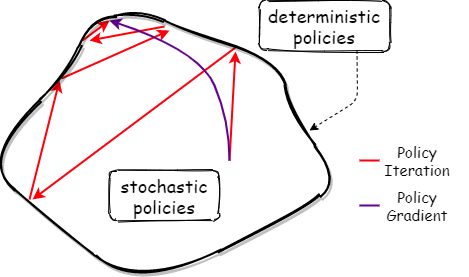
\includegraphics[width=0.35\textwidth]{Images/PGisPI.png}
\vspace{-0.9cm}
\end{wrapfigure}

Это значит, что в текущей точке градиенты указывают туда же, куда и при максимизации $\mathcal{L}_{\textcolor{ChadPurple}{\tilde{\pi}}}(\textcolor{ChadBlue}{\theta})$ по $\textcolor{ChadBlue}{\theta}$. А куда указывает направление градиентов для неё? Выражение $\E_{a \sim \textcolor{ChadBlue}{\pi_{\theta}}(a \mid s)} Q^{\textcolor{ChadPurple}{\tilde{\pi}}}(s, a)$ говорит максимизировать Q-функцию по выбираемым нами действиям: это в чистом виде направление policy improvement-а из теоремы \ref{th:policyimprovement}! 

Но если в табличном сеттинге policy improvement мы делали, так сказать, <<жёстко>>, заменяя целиком стратегию на жадную по действиям, то формула градиента теперь говорит нам, что это лишь направление максимального увеличения $J(\theta)$; после любого шага в этом направлении наша Q-функция тут же, формально, меняется, и в новой точке направление уже должно быть скорректировано. 

Второе уточнение, которое дарит нам эта формула, это распределение, из которого должны приходить состояния. В табличном случае мы не знали, в каких состояниях проводить improvement <<важнее>>, теперь же мы видим, что $s$ должно приходить из $d_{\pi}(s)$. Если какое-то состояние посещается текущей стратегией часто, то улучшать стратегию в нём важнее, чем в состояниях, которые мы посещаем редко.

Это наблюдение, в частности, даёт одно из оправданий тому, что мы отказались от дисконтирования частот посещения состояний. Мы используем формулу градиента для максимизации $V^\pi(s_0)$. Но, в общем-то, мы хотим максимизировать $V^\pi(s)$ сразу для всех $s$, и мы можем делать это с некоторыми весами (и эти веса, в целом, наш произвол). Тогда, выходит, частоты появления $s$ в оптимизируемом функционале определяются в том числе этими весами. Другими словами, $\mu_{\pi}(s)$ указывает на <<самое правильное>> распределение, из которого должны приходить состояния, которые дадут направление именно максимального увеличения функционала, но теория policy improvement-а подсказывает нам, что теоретически корректно выбрать и любое другое.

Получается, исходя из этого рассуждения, что нам для использования формулы градиента даже не нужны on-policy сэмплы, и мы можем брать состояния просто из буфера! Можем ли мы так делать? Допустим, мы готовы заменить распределение состояний на произвольное. Всё равно остаётся существенным сэмплировать действия $a$ именно из текущей версии $\pi(a \HM\mid s)$; значит, брать действие $a$ из буфера нельзя. Следовательно, мы не можем получить $s' \HM\sim p(s' \HM\mid s, a)$; но если у нас как-то есть на руках для любой пары $s, a$ какое-то значение <<кредита>> $Q^\pi(s, a)$, то для градиента актёра нам, согласно формуле, больше ничего и не нужно.

Итак, если у нас есть Q-функция, мы даже с оговорками можем обучать стратегию с буфера, если будем брать из него только состояния, а мат.ожидание по $a$ (или его Монте-Карло оценку) считать, используя текущую стратегию $\pi$. Однако, коли уж мы хотим off-policy алгоритм, то и эту Q-функцию тогда нужно учить с буфера. В итоге, мы получим алгоритм, очень похожий на DQN, со схожими недостатками и преимуществами. Мы обсудим такой подход позже в главе \ref{continuouscontrolchapter}, а пока мы не будем гоняться за возможностью обучаться с буфера и за счёт этого сможем получить некоторые другие полезные преимущества, которые открываются в on-policy режиме.

% Однако, если критик задан V-функцией, то с подсчётом одношаговой аппроксимации \eqref{Qonlineonestep} возникают проблемы: там требуется сэмпл $s' \sim p(s' \mid s, a)$, который в буфере будет записан для произвольного $a$ из буфера из старой стратегии / экспертной стратегии. Поэтому с V-функцией в качестве критика использовать буфер для оптимизации политики не получится: нужны тройки $s, a, s'$, где $a$ сгенерировано онлайн.





